\part{Background}\label{part:background}
\chapter{Quantum Adiabaticity}\label{chap:2_adiabaticity}

\epigraph{``I saw this movie about a bus that had to SPEED around a city, keeping its SPEED over fifty, and if its SPEED dropped, it would explode! I think it was called `The Bus That Couldn’t Slow Down'."}{Homer Simpson, \emph{The Simpsons (S7E10)}}

    
The concept of quantum adiabaticity is the central starting point of the work presented in this thesis. In classical thermodynamics, an adiabatic process is one where no heat is transferred between a system and its environment. On a microscopic quantum mechanical level, this means not changing the occupation/population of Hamiltonian eigenstates. The quantum adiabatic theorem then describes how slowly changes to the Hamiltonian and therefore the eigenstates have to be made so as not to change the distribution. To illustrate, imagine a system that starts in some eigenstate of a Hamiltonian. If a parameter of the Hamiltonian is varied slowly enough, then the system is expected to stay in the corresponding eigenstate of the time-independent `snapshot' Hamiltonian throughout the change and the process is `adiabatic'. In Sec.~\ref{sec:2.1_adiabatic_theorem} we will derive the adiabatic condition and explore what happens when the rate of change in the Hamiltonian parameters is too fast for adiabaticity. As we will find, the non-adiabatic effects that result from fast driving are geometric in nature and related to an operator known as the adiabatic gauge potential \cite{kolodrubetz_geometry_2017, jarzynski_geometric_1995} or \acrref{AGP}, which I will describe in detail in Sec.~\ref{sec:2.2_AGP} and proceed to use it in order to define the concept of counterdiabatic driving \cite{berry_transitionless_2009, demirplak_adiabatic_2003} (\acrref{CD}) in Sec.~\ref{sec:2.3_CD}. \acrref{CD} is a method under the more general umbrella of Shortcuts to Adiabaticity \cite{guery-odelin_shortcuts_2019} (\acrref{STA}), which aim to suppress the non-adiabatic eigenstate deformations that occur when the Hamiltonian parameters are changed too fast, in order to achieve pseudo-adiabatic processes at shorter timescales. In Sec.~\ref{sec:2.4_approximate_CD}, I will demonstrate that exact suppression of non-adiabatic effects in the general case turns out to be impractical (if not impossible) and discuss how one can construct approximate \acrref{CD} protocols which are physically implementable and can mitigate some level of the losses brought about by fast driving.
        
    \section{The quantum adiabatic theorem}\label{sec:2.1_adiabatic_theorem}
    
    Imagine a quantum system that begins in the non-degenerate ground state of a time-dependent Hamiltonian. According to the the quantum adiabatic theorem, it will \emph{remain} in the instantaneous ground state provided the Hamiltonian changes sufficiently slowly (where the meaning of `slow' will become clearer as this section progresses). To take an intuitive example, we can consider a spin in a magnetic field that is rotated from the $x$ direction to the $z$ direction during some total time $\tau$. The Hamiltonian might be written in a chosen basis as:
    \begin{equation}\label{eq:rotating_spin_H}
        H(t) = -\cos\Big(\frac{\pi t}{2 \tau}\Big)\sx - \sin \Big(\frac{\pi t}{2 \tau}\Big)\sz,
    \end{equation}
    with the Pauli matrices defined as:
    \begin{equation}
        \sx = \mqty(0 & 1 \\ 1 & 0), \quad \sy = \mqty(0 & -i \\ i & 0), \quad \sz = \mqty(1 & 0 \\ 0 & -1).  
    \end{equation}
    If the spin starts in the ground state of $H(0)$ (pointing in the $x$ direction, $\ket{\psi(0)} = \ket{+}$), then as the magnetic field is rotated, the spin starts precessing about the new direction of the field. This moves the spin toward the $z$ axis but also produces a component out of the $x-z$ plane. As the total time for the rotation becomes longer (\@i.e.~the rotation gets slower compared to the precession), the state maintains a tighter and tighter orbit around the field direction. In the limit of $\tau \rightarrow \infty$, the state of the spin tracks the magnetic field perfectly, and is always in the ground state of $H(t)$ for all $t$. This is illustrated in Fig.~\ref{fig:bloch_rotating_spin}, which shows the evolution of the system for increasing $\tau$ (and thus decreasing speed). At very fast times, \@e.g.~when $\tau = 1$, the state of the spin veers away from the instantaneous ground state completely, while for $\tau = 50$, the evolution tracks the instantaneous ground state quite closely.
    
    \begin{figure}[t]
    \centering
    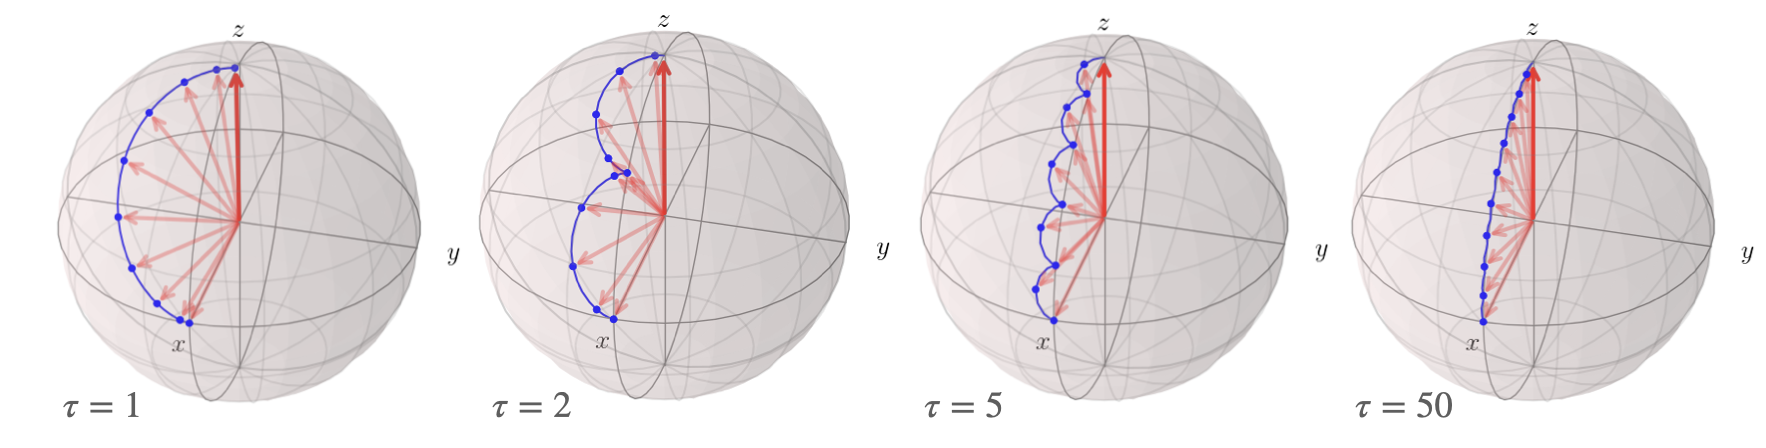
\includegraphics[width=0.9\linewidth]{images/magnetic_field_spin.png} \caption[Rotating spin Bloch sphere illustrations]{Bloch sphere illustration of the single-spin system driven by the Hamiltonian of Eq.~\eqref{eq:rotating_spin_H} for different total driving times $\tau$. The red arrow indicates the ground state of the Hamiltonian at $t = \tau$ while the blue path is that taken by the spin during the evolution.}\label{fig:bloch_rotating_spin}
    \end{figure}

    \subsection{Proof of the adiabatic theorem}\label{sec:2.1.1_proof_adiabatic_theorem}

    The above example gives some intuition for the behaviour of quantum systems as the time of evolution is slowed down, but it doesn't quite answer the question of what it means to be `slow enough' in the general case, \@i.e.~what one would refer to as the \emph{adiabatic condition}. In order to characterise this regime, we first imagine a state $\psi(t)$ which evolves under some time-dependent Hamiltonian $H(t)$. For convenience, we redefine time through the parameter $\lambda = \frac{t}{\tau} \in [0,1]$, such that $\psi(t), H(t) \rightarrow \psi(\lambda), H(\lambda)$ vary smoothly as a function of $\lambda$. This is often done to capture the fact that there may be a natural parameterisation of the changing Hamiltonian such as, for example, two different angles describing a varying magnetic field, which we may want to explore. The parameter space we build generally has some geometric properties that relate to non-adiabatic effects, so it becomes important to talk about these abstract parameters instead of time. But more on this later!
    
    For each value of $\lambda$ throughout the evolution, we have a time-independent `instantaneous' Hamiltonian which can be diagonalised:
    \begin{equation}\label{eq:instantaneous_schroedinger}
        H(\lambda)\ket{n(\lambda)} = E_n(\lambda)\ket{n(\lambda)},
    \end{equation}
    where $E_n(\lambda)$ are the eigenenergies and $\ket{n(\lambda)}$ are the eigenstates. The time-evolution of a system is given by the Schr\"{o}dinger equation $i\hbar \partial_t \ket{\psi(\lambda)} = H(\lambda) \ket{\psi(\lambda)}$ and since the family of eigenvectors $\ket{n(\lambda)}$ constitute a basis at every value of $\lambda$, we can expand the system state as:
    \begin{equation}\label{eq:adiabatic_basis_expansion}
        \ket{\psi(\lambda)} = \sum_n c_n(\lambda)e^{i \dotlambda^{-1} \theta_n(\lambda)}\ket{n(\lambda)},
    \end{equation}
    where $c(\lambda)$ are time-dependent coefficients through the parameter $\lambda$, $\dotlambda = \frac{d\lambda}{dt}$ and
    \begin{equation}\label{eq:dynamical_phase}
        \theta_n(\lambda) = -\frac{1}{\hbar} \int_0^{\lambda} E_n(\lambda') d\lambda'
    \end{equation}
    is commonly referred to as the \emph{dynamic phase}. 
    
    Thus, the task is now to solve the time-dependent Schr\"{o}dinger equation:
    \begin{equation}\label{eq:td-schroedinger}
        i\hbar \dotlambda \ket{\dlambda \psi(\lambda)} = H(\lambda) \ket{\psi(\lambda)},
    \end{equation}
    where $\dlambda$ is the partial derivative with respect to the parameter $\lambda$. We can then use the expansion Eq.~\eqref{eq:adiabatic_basis_expansion}, differentiate and take the inner product with some eigenstate $\bra{m(\lambda)}$ to obtain:
    \begin{equation}\label{eq:adiabatic_derivation}
        \begin{aligned}
         i\hbar \dotlambda \dlambda \sum_n c_n e^{i \dotlambda^{-1} \theta_n} \ket{n} &= H \sum_n c_n e^{i \dotlambda^{-1} \theta_n} \ket{n} \\
        \sum_n \Big( \dlambda c_n \ket{n} + c_n \ket{\dlambda n} + i \dotlambda^{-1} \dlambda\theta_n c_n \ket{n} \Big)e^{i \dotlambda^{-1} \theta_n} &= -\frac{i}{\hbar \dotlambda} \sum_n E_n c_n e^{i \dotlambda^{-1} \theta_n} \ket{n} \\
        \sum_n \Big( \dlambda c_n \ket{n} + c_n \ket{\dlambda n} \Big)e^{i \dotlambda^{-1} \theta_n} &= 0 \\
        \dlambda c_m  &= - \sum_n c_n \braket{m}{\dlambda n}e^{i\dotlambda^{-1}(\theta_m-\theta_n),}
        \end{aligned}
    \end{equation}
    where the last two lines are a consequence of the fact that $i \dotlambda^{-1} \dlambda \theta_n(\lambda) = -\frac{i}{\hbar \dotlambda} E_n(\lambda)$ and the the orthogonality of $\ket{m}$ and $\ket{n}$ when $m \neq n$. Note that I have removed the explicit dependence on $\lambda$ for the sake of readability and to make writing this all out more compact and will continue with this convention for the rest of the chapter unless otherwise stated. 
    
    The above differential equation is exact and describes the evolution of the coefficients $c_n$,  but it doesn't give much of a clue as to what `slow' time evolution means with respect to the changes in the Hamiltonian. For that, we can express the term $\braket{m}{\dlambda n}$ in terms of the changing Hamiltonian. This is done by differentiating Eq.~\eqref{eq:instantaneous_schroedinger} with respect to time and then again taking the inner product with $\bra{m}$ to get:
    \begin{equation}\label{eq:hamiltonian_derivative}
        \begin{aligned}
            \dotlambda \Big(\dlambda{H}\ket{n} + H \ket{\dlambda n}\Big)  &= \dotlambda \Big(\dlambda{E_n}\ket{n} + E_n \ket{\dlambda n}\Big) \\
            \mel{m}{\dlambda H}{n} + \mel{m}{H}{\dlambda n} &= \dlambda E_n\braket{m}{n} + E_n \braket{m}{\dlambda n} \\
            E_m \braket{m}{\dlambda n} - E_n \braket{m}{\dlambda n} &= - \mel{m}{\dlambda H}{n}, \quad m \neq n \\
            \braket{m}{\dlambda n} &= - \frac{\mel{m}{\dlambda H}{n}}{E_m - E_n}, \quad m \neq n
        \end{aligned}
    \end{equation}
    Inserting this into the final line of Eq.~\eqref{eq:adiabatic_derivation}, we find that:
    \begin{equation}\label{eq:coefficient_exact}
            \dlambda c_m + c_m \braket{m}{\dlambda m} = \sum_{n \neq m} c_n  \frac{\mel{m}{\dlambda H}{n}}{E_m - E_n}e^{i \dotlambda^{-1} (\theta_m-\theta_n)}.
    \end{equation}
    
    When the term on the RHS is small, which is a condition that will be discussed in more detail in the next section, we can neglect it and the solution for the remaining differential equation of $c_m$ is just:
    \begin{equation}\label{eq:c_adiabatic}
        c_m(\lambda) = c_m(0)e^{i \gamma_m(\lambda)},
    \end{equation}
    where
    \begin{equation}\label{eq:geometric_phase}
        \gamma_m(\lambda) = i \int_0^{\lambda} \braket{m}{\partial_{\lambda'} m} d \lambda' 
    \end{equation}
    is the geometric (or Berry) phase \cite{pancharatnam_generalized_1956, longuet-higgins_studies_1958, berry_quantal_1984}. It arises from the fact that if the Hamiltonian varies according to $\lambda$ in a closed loop way, \@i.e.~it returns to its starting point at the end of the evolution, the wavefunction might not. Think of Foucault's pendulum, which changes its plane of swinging due to the Earth's rotation around its own axis and does not necessarily return to its initial state after a full rotation. Both the appearance of the geometric phase in Eq.~\eqref{eq:c_adiabatic} and the changing plane of Foucault's pendulum are consequences of the geometry or `curvature' of the parameter space in which the dynamics occur and are related to concepts like parallel transport. To illustrate this, we can absorb the geometric phase into the adiabatic eigenstates via the transformation
    \begin{equation}\label{eq:parallel_transport_state}
        \ket{m'} = e^{i \gamma_m(\lambda)}\ket{m} = e^{- \int_0^{\lambda} \braket{m}{\partial_{\lambda'} m} d \lambda'}\ket{m},
    \end{equation}
    and then take the derivative of the above expression with $\lambda$ followed by taking the inner product with $\bra{m'}$. This gives:
    \begin{equation}\label{eq:geometric_phase_cancellation}
        \braket{m'}{\dlambda m'} = 0,
    \end{equation}
    which in other words just means that some change in the parameter $\lambda$ produces an eigenvector that is orthogonal to the unchanged eigenstate. This turns out to be the condition which defines parallel transport along a curve in a curved space, as analogous to the classical example of Foucault's pendulum. The choice of phases in Eq.~\eqref{eq:parallel_transport_state} is generally referred to as the \emph{parallel transport gauge}\cite{nakahara_geometry_2003}.
    
    The constraint that the RHS of Eq.~\eqref{eq:coefficient_exact} be negligible is exactly the adiabatic condition, which can be seen by checking that $\abs{c_m(\lambda)}^2 = \abs{c_m(0)}^2$ in Eq.~\eqref{eq:c_adiabatic}. What this means is that a state starting in a particular eigenstate $\ket{m(\lambda)}$ will remain in that state under these circumstances, \@e.g.~for $c_m(0) = 1$ and $c_{m \neq n}(0) = 0$:
    \begin{equation}\label{eq:adiabatic_states}
        \ket{\psi(\lambda)} = e^{i \dotlambda^{-1} \theta_m(\lambda)}e^{i \gamma_m(\lambda)} \ket{m(\lambda)}
    \end{equation}
    the $m^{\text{th}}$ eigenstate stays in the $m^{\text{th}}$ eigenstate.
    
    So to understand adiabaticity, we need to understand what conditions lead to the case where
    \begin{equation}\label{eq:adiabaticity_condition}
        \sum_{n \neq m} c_n \frac{\mel{m}{\dlambda H}{n}}{E_m - E_n}e^{i \dotlambda^{-1} (\theta_m-\theta_n)} \ll 1,
    \end{equation}
    which is exactly what the next section sets out to do.
    
    \subsection{The adiabatic condition: how slow is \emph{slow}?}\label{sec:2.1.2_adiabatic_condition}

    The condition given by Eq.~\eqref{eq:adiabaticity_condition} contains terms relating both to the rate of change of the Hamiltonian with respect to $\lambda$ (expressed in terms of matrix elements $\mel{m}{\dlambda H}{n}$) and the energy gap between eigenstates $E_m - E_n$. It is not too hard to see that when the energy gaps are very large, these terms can be neglected. However, let us try to derive a more concrete and quantitative measure for `slowness'.

    First, we can go back to the intermediate result from Eq.~\eqref{eq:coefficient_exact} and write it out as:
    \begin{equation}\label{eq:perturbative_adiabatic}
        \dlambda c_m = \sum_n c_n \braket{m}{\dlambda n}e^{i\dotlambda^{-1}(\theta_m - \theta_n)}.
    \end{equation}
    Since we want to focus on the RHS terms where $m \neq n$, we can remove the $m = n$ term by a change of variables:
    \begin{equation}\label{eq:changing_variables}
        d_m = c_m e^{\int_0^{\lambda}\braket{m}{\dlambda m} \dlambda} = c_m e^{-i\gamma_m}
    \end{equation}
    and then, using Eq.~\eqref{eq:perturbative_adiabatic}, we find
    \begin{equation}\label{eq:n_neq_m_terms}
        \begin{aligned}
            \dlambda d_m &= - \sum_n c_n \braket{m}{\dlambda n}e^{i\dotlambda^{-1}(\theta_m - \theta_n)}e^{-i\gamma_m} + c_m \braket{m}{\dlambda m} e^{-\gamma_m} \\
            &= - \sum_{n \neq m} d_n \braket{m}{\dlambda n} e^{-i(\gamma_m - \gamma_n)} e^{i\dotlambda^{-1}(\theta_m - \theta_n)} \\
            \Rightarrow{} e^{i\gamma_m} \dlambda(c_m e^{-i\gamma_m}) &= - \sum_{n \neq m} c_n \braket{m}{\dlambda n} e^{i \gamma_n} e^{i\dotlambda^{-1}(\theta_m - \theta_n)}
        \end{aligned}
    \end{equation}
    Now all that is left is integration, which leads to:
    \begin{equation}\label{eq:adiabatic_coefficients_dyanmics}
        c_m(1)e^{-i\gamma_m} = c_m(0) - \int_0^1 \sum_{n \neq m} c_n \braket{m}{\dlambda n} e^{i\dotlambda^{-1}(\theta_m - \theta_n)} e^{i(\gamma_n - \gamma_m)} d \lambda.
    \end{equation}

    In the above, we can see that when the integral on the RHS is 0, we recover the result in Eq.~\eqref{eq:c_adiabatic}. The intuition is that when the integral is sufficiently small, the adiabatic condition is valid and the system will follow the instantaneous eigenstate. Since the integral is made up of a sum of terms of the same form, we can focus on determining the bound on one of them. Representing the integral as:
    \begin{equation}\label{eq:adiabatic_integral_main}
        I_{n \neq m}(1) = \int_0^1 c_n \frac{\mel{m}{\dlambda H}{n}}{E_m - E_n} e^{i\dotlambda^{-1}(\theta_m - \theta_n)} e^{i(\gamma_n - \gamma_m)} d \lambda,
    \end{equation}
    where we used the result from Eq.~\eqref{eq:hamiltonian_derivative}. The integral doesn't can be simplified a lot by using the fact that:
    \begin{equation}
        \begin{aligned}\label{eq:simplifying_adiabatic_integral}
            \dlambda \left( c_n(\lambda) \frac{A_{m,n}(\lambda)}{\omega_{m,n}^2(\lambda)}e^{i\dotlambda^{-1}(\theta_m - \theta_n)} \right) = &\dlambda \left( c_n(\lambda) \frac{A_{m,n}(\lambda)}{\omega_{m,n}^2(\lambda)}\right) e^{i\dotlambda^{-1}(\theta_m - \theta_n)} \\ &- \frac{i}{\hbar \dotlambda} c_n(\lambda) \frac{A_{m,n}(\lambda)}{\omega_{m,n}(\lambda)}e^{i\dotlambda^{-1}(\theta_m - \theta_n)} \\ 
            \Rightarrow c_n(\lambda) \frac{A_{m,n}(\lambda)}{\omega_{m,n}(\lambda)}e^{i\dotlambda^{-1}(\theta_m - \theta_n)} = &-i\hbar\dotlambda \Bigg[ \dlambda \left(c_n(\lambda) \frac{A_{m,n}(\lambda)}{\omega_{m,n}^2(\lambda)} \right) e^{i\dotlambda^{-1}(\theta_m - \theta_n)} \\
            &- \dlambda \left( c_n(\lambda) \frac{A_{m,n}(\lambda)}{\omega_{m,n}^2(\lambda)}e^{i\dotlambda^{-1}(\theta_m - \theta_n)} \right) \Bigg],
        \end{aligned}
    \end{equation}
    where I have used $A_{m,n}(\lambda) = \mel{m(\lambda)}{\dlambda H(\lambda)}{n(\lambda)}e^{-i(\gamma_m(\lambda) - \gamma_n(\lambda))}$ and $\omega_{m,n}(\lambda) = E_m(\lambda) - E_n(\lambda)$. This result can now be inserted into Eq.~\eqref{eq:adiabatic_integral_main}, leading to:
    \begin{equation}\label{eq:final_adiabatic_integral}
        \begin{aligned}
            I_{n \neq m}(1) = \: &i\hbar \dotlambda \left[ c_n(\lambda) \frac{A_{m,n}(\lambda)}{\omega_{m,n}^2(\lambda)} e^{-\frac{i}{\hbar \dotlambda}\int_0^{\lambda}\omega_{m,n}(\lambda')d \lambda'}  \right]_0^1 \\ 
            \quad &-i\hbar \dotlambda \int_0^1 \frac{d}{d\lambda'} \left(c_n(\lambda) \frac{A_{m,n}(\lambda)}{\omega_{m,n}^2(\lambda)} \right) e^{-\frac{i}{\hbar \dotlambda}\int_0^{\lambda'}\omega_{m,n}(\lambda'')d \lambda''} \\
            \approx &-i\hbar \dotlambda \left[ c_n(1) \frac{A_{m,n}(1)}{\omega_{m,n}^2(1)}e^{-\frac{i}{\hbar \dotlambda}\int_0^{1}\omega_{m,n}(\lambda')d \lambda'} - c_n(0) \frac{A_{m,n}(0)}{\omega_{m,n}^2(0)} \right] \\
            = &-i\hbar \dotlambda c_n(1) \frac{A_{m,n}(1)}{\omega_{m,n}^2(1)}e^{-\frac{i}{\hbar \dotlambda}\int_0^{1}\omega_{m,n}(\lambda')d \lambda'},
        \end{aligned}
    \end{equation}
    where the last line is a consequence of the assumption that the that the system starts in the eigenstate $m$, and thus at $\lambda = 0$, the coefficient $c_{n \neq m} = 0$. As for the disappearing integral on the second line, this is due to the fact that $\dotlambda = \frac{1}{\tau}$ and at long times $\tau \rightarrow \infty$, when the adiabatic condition is supposed to hold, the integrand will oscillate so fast that it will effectively vanish\cite{kahane_generalizations_1980}. 

    The term we're left with can effectively be bounded from above, since both exponential terms $e^{-\frac{i}{\hbar \dotlambda}\int_0^{1}\omega_{m,n}(\lambda')d \lambda'}$ and $e^{-i(\gamma_m(\lambda) - \gamma_n(\lambda))}$ (which has been absorbed into $A_{n,m}(\lambda)$) have a maximal value of 1. The same goes for $c_n(1)$. This leaves us with a bound on the remaining quantities:
    \begin{equation}\label{eq:adiabatic_criterion}
        \max _{n,m}\left[\max_{\lambda} \left| \frac{\hbar \dotlambda \mel{m(\lambda)}{\dlambda H(\lambda)}{n(\lambda)}}{(E_m(\lambda) - E_n(\lambda))^2} \right| \right] \ll 1, \quad m \neq n,
    \end{equation}
    which is exactly the adiabatic condition, as expected. 

    To illustrate the point more clearly, we can look back to the example Hamiltonian of Eq.~\eqref{eq:rotating_spin_H}, where the energy gap between the two eigenstates $\ket{\psi_1(t)}$ and $\ket{\psi_2(t)}$ is a constant: $E_{\psi_1} - E_{\psi_2} = 2$, and so are the matrix elements $\mel{\psi_1}{\dot{H}}{\psi_2} = \mel{\psi_2}{\dot{H}}{\psi_1} = \frac{\pi}{2 \tau}$. The dependence on $\tau$ of the off-diagonal matrix elements of $\dot{H}$ make the results of Fig.~\ref{fig:bloch_rotating_spin} immediately clearer: as $\tau$ increases (and hence the evolution is slower), the non-adiabatic component of Eq.~\eqref{eq:adiabatic_criterion} decreases proportionately to it. More details on the example and the derivation can be found in Appendix \ref{app:rotating_spin_hamiltonian}.

     In practice, it is not immediately obvious how the quantity stated in Eq.~\eqref{eq:adiabatic_criterion} relates to, say, the fidelity of the final state with respect to the desired state or how large $\tau$, the evolution time, has to be in order to lead to a fidelity of some magnitude. While it is possible to find these bounds, the proof is quite lengthy and not necessary for the purposes of this thesis, so instead I will refer you to \cite{reichardt_quantum_2004, childs_lecture_2008} for more details.
    
    \section{The adiabatic gauge potential}\label{sec:2.2_AGP}

    The previous section introduced quantum adiabaticity and presented some intuition for non-adiabatic effects at fast driving times. In this section, I want to establish the deeply related concept of the adiabatic gauge potential (\acrref{AGP}) \cite{kolodrubetz_geometry_2017}, a key player in the subject matter of this thesis and a fascinating mathematical object in its own right. While the \acrref{AGP} has primarily been studied in the context of suppressing non-adiabatic effects \cite{sels_minimizing_2017, claeys_floquet-engineering_2019}, as will be its central role in this thesis, in recent years it has also been shown to be a potential probe for quantum chaos \cite{pandey_adiabatic_2020} and has been proposed for the study of thermalisation \cite{nandy_delayed_2022}. These results are possible because quantum chaos manifests itself through exponential sensitivity of the eigenstates to infinitesimal perturbations that are generated by the \acrref{AGP}, making the scaling of its norm a very sensitive probe for quantum chaos and thermalisation.

    \subsection{The moving frame Hamiltonian}

    In Section \ref{sec:2.1.1_proof_adiabatic_theorem} we spent some time working in the instantaneous eigenbasis of the Hamiltonian where it is diagonalised, à la Eq.~\eqref{eq:instantaneous_schroedinger}. For a general Hamiltonian, it is possible to go to this `moving frame' picture by rotating the Hamiltonian via some unitary $U$ so that it becomes diagonal at each point in time. If we start with some arbitrary Hamiltonian $H(\lambda)$ in some sort of `lab frame' that depends on time through the parameter(s) $\lambda(t)$, it can be diagonalised through $\Tilde{H} = U^{\dagger}(\lambda)H(\lambda)U(\lambda)$, where the $\sim$ implies that we are now in the basis of the moving frame. In general, whenever the tilde symbol appears above an operator throughout this section, it means that we are working in this new basis: $\Tilde{\sigma} = \adj{U}\sigma U$.

    We can also view the quantum system evolving under the Hamiltonian in this moving frame picture: $\ket*{\Tilde{\psi}} = U^{\dagger}\ket{\psi}$, which is equivalent to expanding the wave function in the moving frame (or instantaneous) basis exactly as was done in Eq.~\eqref{eq:adiabatic_basis_expansion}. Given this new basis, rewriting the Schr\"{o}dinger equation reveals something interesting:
    \begin{equation}\label{eq:moving_frame_schrodinger}
        \begin{aligned}
            i \hbar \frac{d \ket*{\Tilde{\psi}}}{dt} &= i \hbar \Big( \frac{d \adj{U}}{dt}\ket*{\psi} + \adj{U} \frac{d \ket{\psi}}{dt} \Big) \\
            &= i \hbar \dotlambda \frac{\partial \adj{U}}{\partial \lambda}\ket{\psi} + \adj{U} H\ket{\psi}\\
            &= \dotlambda \Big(i\hbar \frac{\partial \adj{U}}{\partial \lambda}U \Big)\ket*{\Tilde{\psi}} + \adj{U} H U \ket*{\Tilde{\psi}} \\
            &= \Big(\Tilde{H} - \dotlambda\Tilde{\AGP{\lambda}}\Big) \ket*{\Tilde{\psi}},
        \end{aligned}
    \end{equation}
    where the operator $\Tilde{\AGP{\lambda}}$ is the \emph{adiabatic gauge potential} with respect to the parameter $\lambda$ in the moving frame of the Hamiltonian $H$ and is expressed as:
    \begin{equation}\label{eq:AGP_in_terms_of_U}
        \Tilde{\AGP{\lambda}} = i\hbar \adj{U}\dlambda U.
    \end{equation}
    
    The name `gauge potential' refers to operators that are generators of continuous unitary translations in parameter space \cite{kolodrubetz_geometry_2017} of some unitary transformation $U$ and generally takes the form of a derivative operator. In fact, the name originates from quantities under which the physics is invariant. For example, the gauge potential responsible for translations in space is just the momentum operator $p = i\hbar \partial_x$. This can be illustrated in the case of the simple 1D harmonic oscillator with a moving potential centered on $x_0(t)$:
    \begin{equation}\label{eq:harmonic_oscillator}
        H(x_0) = \frac{p^2}{2m} + \frac{1}{2}m \omega^2 (x - x_0)^2,
    \end{equation}
    which can be diagonalised with the transformation $U(x_0) = e^{-i p x_0/\hbar}$. Then the gauge potential is simply:
    \begin{equation}
        \Tilde{\AGP{\lambda}} = i\hbar e^{i p x_0/\hbar} \dlambda e^{-i p x_0/\hbar} = p.
    \end{equation}
    
    In this thesis we will restrict ourselves to the specific case of adiabaticity where the transformation $U(\lambda)$ explicitly takes a wavefunction in an arbitrary basis to the adiabatic or instantaneous basis. 
    
    So what we find is that the wavefunction in the moving frame basis evolves under a combination of the diagonal component $\Tilde{H}$ and some additional term proportional both to the speed at which the parameter $\lambda$ varies and the \acrref{AGP}. At this point I would like to simplify things by largely getting rid of the $\sim$, which we can do by applying the inverse unitary operation in order to work back in lab frame basis: $\Tilde{H} - \dotlambda\Tilde{\AGP{\lambda}} \xrightarrow{U \{ \cdot \} \adj{U}} H - \dotlambda \AGP{\lambda}$. In fact, this transformation makes it easy to see how we can think of the AGP in the lab frame as nothing more than the derivative operator: $\AGP{\lambda} = i\hbar\dlambda$. 

    To see this, take any quantum state written in some basis, \@e.g.~$\ket{\psi} = \sum_n \psi_n \ket{n}$. Then in the moving frame basis we have:
    \begin{equation}\label{eq:AGP_basis_change}
            \ket{\psi} = \sum_n \psi_n \adj{U}(\lambda) \ket{n} = \sum_{\Tilde{n}} \Tilde{\psi}_n (\lambda) \ket*{\Tilde{n}(\lambda)},
    \end{equation}
    where $\Tilde{\psi}_n (\lambda) = \sum_n \adj{U}(\lambda) \psi_n = \braket{\Tilde{n}(\lambda)}{\psi}$ and the dependence on $\lambda$ enters into the basis vectors through the rotation $U(\lambda)$. These two bases can now allow us to look at the matrix elements of $\AGP{\lambda}$ in both:
    \begin{equation}\label{eq:AGP_as_derivative}
        \begin{aligned}
            \mel{n}{\Tilde{\AGP{\lambda}}}{m} &= \mel{n}{i\hbar \adj{U}\dlambda U}{m} \\
            &= i\hbar \mel{\Tilde{n}(\lambda)}{\dlambda}{\Tilde{m}(\lambda)} \\
            &= \mel{\Tilde{n}(\lambda)}{\AGP{\lambda}}{\Tilde{m}(\lambda)}
        \end{aligned}
    \end{equation}
    where the last line is simply the statement that in the lab frame $\AGP{\lambda} = i\hbar \dlambda$.

    \subsection{Matrix elements of the AGP}

    What we have seen so far is that when we try to solve the Schr\"{o}dinger equation for a quantum system evolving under a time-dependent Hamiltonian in the basis of the moving frame, \@i.e.~in the basis where the time-dependent Hamiltonian is diagonalised, we find that the evolution happens under a `decorated' Hamiltonian composed of the diagonalised $\Tilde{H}$ and an additional operator generally known as the adiabatic gauge potential or \acrref{AGP}. We found that in the lab frame, it is the derivative operator with respect to the time-dependent parameters driving the Hamiltonian. What remains is to link this to our discussion of adiabaticity and the adiabatic condition of Section \ref{sec:2.1_adiabatic_theorem}.

    Let us return to the matrix elements of the lab frame \acrref{AGP} and see what they are in the adiabatic basis of Eq.~\eqref{eq:instantaneous_schroedinger}, which is the eigenbasis of the instantaneous Hamiltonian. The first thing that jumps out is that the diagonal elements of the \acrref{AGP} are very familiar:
    \begin{equation}\label{eq:AGP_diagonal}
        \mel{n(\lambda)}{\AGP{\lambda}}{n(\lambda)} = i\hbar \mel{n(\lambda)}{\dlambda}{n(\lambda)}.
    \end{equation}
    The terms on the RHS are something known as the Berry connections and they look familiar because they are the integrands of the geometric phase (Eq.~\eqref{eq:geometric_phase}) that we found when deriving the adiabatic condition. I mentioned that the geometric phase is related to the geometry or curvature of the parameter space of the adiabatic Hamiltonian and the \acrref{AGP} contains information about this geometry. 

    In order to understand what the off-diagonal elements of the AGP are, we can make use of the fact that in the instantaneous Hamiltonian basis $\mel{m}{H}{n} = 0$ for $m \neq n$. Differentiating with respect to the parameter $\lambda$ gives:
    \begin{equation}\label{eq:differentiating_adiabatic_offdiagonals}
       \begin{aligned}
           \mel{\dlambda m}{H}{n} + \mel{n}{\dlambda H}{n} + \mel{n}{H}{\dlambda m} &= 0 \\
           E_n \braket{\dlambda m}{n} + E_m \braket{m}{\dlambda n} + \mel{n}{\dlambda H}{n} &= 0 \\
           (E_m - E_n) \braket{m}{\dlambda n} + \mel{n}{\dlambda H}{n} &= 0 \\
           \frac{-i}{\hbar} (E_m - E_n) \mel{m}{\AGP{\lambda}}{n} + \mel{n}{\dlambda H}{n} &= 0 \\
           \mel{m}{\AGP{\lambda}}{n} &= i\hbar \frac{\mel{m}{\dlambda H}{n}}{(E_n - E_m)},
       \end{aligned} 
    \end{equation}
    where, since we're working in the adiabatic basis, all eigenstates, eigenenergies and the operators depend on $\lambda$. We can now see that $\AGP{\lambda}$ is Hermitian and the final line is familiar: the off-diagonal elements of the \acrref{AGP} are proportional to the non-adiabatic contribution we derived back in Eq.~\eqref{eq:final_adiabatic_integral}. The full operator in the adiabatic basis is:
    \begin{equation}\label{eq:AGP_adiabatic_basis}
        \AGP{\lambda} = i\hbar\Big(\sum_n \braket{n}{\dlambda n} \dyad{n} + \sum_{m \neq n} \ket{m} \frac{\mel{m}{\dlambda H}{n}}{(E_n - E_m)} \bra{n} \Big).
    \end{equation}

    The outcome of this section then, is the revelation that this (initially mysterious) operator known as the \acrref{AGP} is deeply linked to the notion of adiabaticity in quantum systems: its diagonal terms are related to the geometry of the parameter space of adiabatic dynamics while its off-diagonals elements describe the non-adiabatic eigenstate deformations experienced by a state when it is driven by a time-dependent Hamiltonian. It is useful to note that in the final line of Eq.~\eqref{eq:moving_frame_schrodinger} we found that the Schr\"{o}dinger equation corresponding to the evolution of the instantaneous eigenstates is:
    \begin{equation}\label{eq:schrodinger_moving_frame_2}
        i \hbar \frac{d \ket*{\Tilde{\psi}}}{dt} = \Big( \Tilde{H} - \dotlambda \AGP{\lambda} \Big) \ket*{\Tilde{\psi}},
    \end{equation}
    where now it is not difficult to find how each of these operators contributes to the results of Section \ref{sec:2.1.1_proof_adiabatic_theorem}. The moving frame or instantaneous Hamiltonian generates the dynamical phase factor in Eq.~\eqref{eq:dynamical_phase}, the diagonal elements of the \acrref{AGP} produce the geometric phase factor given by Eq.~\eqref{eq:geometric_phase} and the off-diagonal elements of \acrref{AGP} are responsible for the non-adiabatic transitions out of the eigenstates which we upper bounded in Section \ref{sec:2.1.2_adiabatic_condition}. For a more detailed proof of how to derive the adiabatic theorem starting from Eq.~\eqref{eq:schrodinger_moving_frame_2} I recommend \cite{petiziol_accelerated_2020}.
    
    \section{Counterdiabatic Driving}\label{sec:2.3_CD}

    Having done all this work to characterise and understand the \acrref{AGP} and the adiabatic theorem, we now come to several important questions, starting with \emph{why do we care}? What is it about adiabatic dynamics that makes them important? Why do we want to quantifying non-adiabatic transformations and understand what generates? The answer is simple: adiabatic processes are useful. The ability to drive a time-dependent Hamiltonian while remaining in a particular eigenstate can be used to prepare interesting quantum states \cite{dimitrova_many-body_2023}, to solve combinatorics problems encoded in quantum systems \cite{ebadi_quantum_2022, pichler_quantum_2018} or even to synthesise effective ramps and quantum logic gates \cite{pelegri_high-fidelity_2022} among many other applications. 
    
    The most natural way of exploiting adiabatic protocols is by adhering to the adiabatic condition. However, as is often the case when it come to the control of quantum systems, things aren't quite that simple. In practice, changing a Hamiltonian slowly enough to satisfy Eq.~\eqref{eq:adiabatic_criterion} leads to the system being overwhelmed by decoherence in many cases. Furthermore, as system sizes get larger, the energy gaps between the instantaneous eigenstates tend to get smaller requiring slower and slower driving, making adiabatic protocols unscalable. While the adiabatic condition is not impossible to adhere to, in order to have any hope of pushing quantum technologies beyond their current limits, it is necessary to move beyond the adiabatic limit. The result is that we need to find ways to achieve the same results as adiabatic processes but without requiring the prohibitively long driving times that are demanded by Eq.~\eqref{eq:adiabatic_criterion}.
    
    Our analysis of the adiabatic condition has given us a clue as to how we might be able to achieve fast driving without the eigenstate deformations that result from fast driving. Returning to Eq.~\eqref{eq:adiabatic_states}, we may focus our attention on the fact that our goal is simply to have the system follow the eigenstates of the instantaneous Hamiltonian. The approach that aims to do exactly this was first developed independently by Demirplak and Rice \cite{demirplak_adiabatic_2003} and Berry \cite{berry_transitionless_2009} and began as the observation that one can attempt to reverse-engineer a Hamiltonian that drives the instantaneous eigenstates exactly. Recall from Eq.~\eqref{eq:adiabatic_states} that in the case that we have adiabatic evolution, the instantaneous eigenstates evolve as $\ket{\psi(\lambda)} = e^{i \dotlambda^{-1} \theta_m(\lambda)}e^{i \gamma_m(\lambda)} \ket{m(\lambda)}$ with the dynamical phase $\theta_m$ and geometric phase $\gamma_m$ defined in Eq.~\eqref{eq:dynamical_phase} and Eq.~\eqref{eq:geometric_phase} respectively. If we want to find a Hamiltonian $H_{\rm t-less} (\lambda)$ (transitionless) that drives these states exactly, we can pick a unitary $R(\lambda)$ such that:
    \begin{equation}
        \begin{aligned}
            i\hbar \dotlambda \partial_{\lambda} R(\lambda) &= H_{\rm t-less} (\lambda) R(\lambda), \\
            \Rightarrow H_{\rm t-less} (\lambda) &= i\hbar \dotlambda (\partial_{\lambda} R(\lambda)) \adj{R}(\lambda).
        \end{aligned}
    \end{equation}
    It turns out this unitary is just:
    \begin{equation}\label{eq:transitionless_unitary}
        R(\lambda) = \sum_m e^{i \dotlambda^{-1} \theta_m(\lambda)}e^{i \gamma_m(\lambda)} \dyad{m(\lambda)}{m(0)},
    \end{equation}
    so the transitionless Hamiltonian can be expressed as:
    \begin{equation}
        \begin{aligned}\label{eq:transitionless_hamiltonian}
            \begin{aligned}
                H_{\rm t-less}(\lambda) = \: &i \hbar \dotlambda \sum_m \Bigg[ \Big(- \frac{i E_m}{\dotlambda \hbar} - \braket{m(\lambda)}{\dlambda m(\lambda)}\Big) e^{i \dotlambda^{-1} \theta_m(\lambda)}e^{i \gamma_m(\lambda)} \dyad{m(\lambda)}{m(0)} \\
                &+ e^{i \dotlambda^{-1} \theta_m(\lambda)}e^{i \gamma_m(\lambda)} \dyad{\dlambda m(\lambda)}{m(0)} \Bigg] e^{-i \dotlambda^{-1} \theta_m(\lambda)}e^{-i \gamma_m(\lambda)} \dyad{m(0)}{m(\lambda)} \\
                 = &\sum_m \ket{m} E_m \bra{m} + i\hbar \dotlambda \sum_m (\dyad{\dlambda m}{m} - \braket{m}{\dlambda m} \dyad{m}),
            \end{aligned}
        \end{aligned}
    \end{equation}
    where in the last line the dependence on $\lambda$ has once again been removed from the eigenstates $\ket{m}$ and the eigenenergies $E_m$ noting that all terms for $\lambda = 0$ have been cancelled out. In order to analyse the equation more easily, I'll rewrite it in terms of two separate components:
    \begin{equation}\label{eq:transitionless_h0_h1}
        H_{\rm t-less}(\lambda) = H_0(\lambda) + H_1(\lambda),
    \end{equation}
    where 
    \begin{equation}
        \begin{aligned}
            H_0 &= \sum_m E_m \dyad{m}, \\
            H_1 &= i\hbar \dotlambda \sum_m (\dyad{\dlambda m}{m} - \braket{m}{\dlambda m} \dyad{m}).
        \end{aligned}
    \end{equation}

    What the above equation shows is that if we can engineer the Hamiltonian $H_{\rm t-less} (\lambda)$, it is possible to drive the system arbitrarily fast, as it will always follow the instantaneous eigenstates. This might seem like a strange statement, but it becomes a lot simpler when we consider that the term $H_1$ looks quite familiar: it is nothing more than the negation of the \acrref{AGP} component in Eq.~\eqref{eq:schrodinger_moving_frame_2}. You may have already noticed that what Eq.\eqref{eq:transitionless_hamiltonian} is actually doing in the moving frame is simply:
    \begin{equation}\label{eq:AGP_cancelling_out}
    	(\Tilde{H} - \dotlambda \Tilde{\AGP{\lambda}}) + \dotlambda \Tilde{\AGP{\lambda}} = \Tilde{H},
    \end{equation}
    which is reflected in the fact that $H_1$ is nothing more than the non-adiabatic contribution generated by the \acrref{AGP}. In the equation above, the effective Hamiltonian in the moving frame is simply the diagonalized version of the driving Hamiltonian $H(\lambda)$ in the lab frame, which does nothing more than drive the instantaneous eigenstates perfectly. This is the idea behind \emph{counterdiabatic driving} or \acrref{CD}. The name, unsurprisingly, stems from the fact that the additional `counterdiabatic' term $+ \dotlambda\AGP{\lambda}$ is added in order to `counter' the non-adiabatic or `diabatic' effects that arise in the effective Hamiltonian throughout the system's evolution.
    
    Since all of the operators in the above equation are in the moving frame basis, we can rotate them back to the lab frame and explicitly define the counterdiabatic Hamiltonian:
    \begin{equation}\label{eq:CD_Hamiltonian}
    \HCD(\lambda) = H(\lambda) + \dotlambda \mathcal{A}_\lambda,
    \end{equation}
    where we recall from Eq.~\eqref{eq:moving_frame_schrodinger} that $H(\lambda)$ becomes an effective $\Tilde{H} - \dotlambda \Tilde{\AGP{\lambda}}$ in the moving frame.

    This seems simple enough: if $\HCD$ is known and can be engineered, it is possible to drive a quantum system arbitrarily fast with no deformations associated with non-adiabatic effects. However, if this seems too good to be true, that's because in general it is. The first clue is in the form of the \acrref{AGP} in Eq.~\eqref{eq:AGP_adiabatic_basis}, which implies that in order to know this \acrref{CD} Hamiltonian, we'd need to not only know the full eigenspectrum of the lab frame Hamiltonian for each value of $\lambda$ throughout the protocol, but also to be able to engineer such terms to arbitrary precision in the lab. Furthermore, the off-diagonal elements of $\AGP{\lambda}$, as alluded to earlier, are proportional to the inverse of the energy gaps in the system $(E_n - E_m)$, which become exponentially small as system sizes increase and can become divergent or undefined in the thermodynamic limit \cite{kolodrubetz_geometry_2017, jarzynski_geometric_1995}. In chaotic systems, the \acrref{AGP} cannot be local because no local operator can distinguish many-body states with arbitrary small energy difference \cite{dalessio_quantum_2016}. What all of this really implies is that it is impossible - or at least impractical - to attempt to implement the exact counterdiabatic Hamiltonian given by Eq.~\eqref{eq:CD_Hamiltonian} in the general case, barring some very simple and small systems.

    \subsection{Brief interlude: the waiter and the glass of water}

    It may seem like our inability to know or implement the exact \acrref{CD} Hamiltonian of Eq.~\eqref{eq:CD_Hamiltonian} in the general case brings us back to square one in trying to speed up adiabatic protocols. I will show in the next section that it turns out this is not the case at all. However, before I dive back into the math, I wanted to take a moment to illustrate the concept of \acrref{CD} with a classical analogy which I first encountered in \cite{sels_minimizing_2017} and which I think not only elucidates what we've talked about so far, but also gives some intuition for how we might overcome the practical problems associated with the exact \acrref{AGP}, setting the stage nicely for the rest of the chapter.
    
    The story goes something like this: imagine that you are a waiter tasked with carrying a glass of water on a tray from the bar to some table on the other side of a rather large restaurant. As you begin to walk while holding the tray perfectly level with the ground, your acceleration induces a force on the glass which causes it to wobble and the water to splash around. Ideally you would like to stop the water from spilling, so at this point you have two options: either to (a) walk slowly so as to minimize the force that is destabilizing the glass or else (b) to counteract it by tilting the tray. 

    You may already see where we are going with this. In the analogy, we can view the stable, upright state of the glass full of water as the ground state of some quantum system. The moving waiter then embodies the time-dependent Hamiltonian, where we can model their changing coordinates as they move through the bar via the abstract parameter(s) $\lambda$. Just as in the case of the adiabatic condition of Eq.~\eqref{eq:adiabatic_criterion}, the chance of the glass tipping over depends on both the acceleration and direction of the waiter (the $\dlambda H$ term) as well as how inherently stable the glass is due to \@e.g.~a heavier bottom or more viscous liquid (the energy gap between the ground state and the nearest excited state). In this picture, the two methods the waiter can use to stabilize the glass during transport are analogous to (a) following the adiabatic condition by minimizing the speed at which the Hamiltonian is deformed or (b) applying counterdiabatic driving \@i.e.~counteracting the non-adiabatic force that appears as a consequence of their fast movement.
    
    This example is not only useful for gaining intuition about adiabaticity and \acrref{CD}, but can also be used to bring attention to several interesting observations. The first is that by including a counterdiabatic component, the waiter introduces a new degree of freedom - a tilt - which would otherwise not show up anywhere in the process or the start/end points of the journey of the glass. Secondly, from the point of view of someone standing by the wayside (the lab frame), the glass is nowhere near standing upright throughout the counterdiabatic tilt, rather it is in some highly excited state, while from the perspective of the glass (the moving frame) it is quite stable and generally close to the instantaneous ground state, as can be garnered from looking at Equations \eqref{eq:AGP_cancelling_out} and \eqref{eq:CD_Hamiltonian} as representative of the two perspectives. The most important observation, however, which springboards us into the next section of this chapter, is precisely one which answers the question: \emph{how stable is the glass throughout the waiter's counterdiabatic journey}? We cannot assume, in any realistic scenario, that the waiter has perfect knowledge of the movement of every molecule of water in the glass and can control their movements to such high precision that they instantly counteract even the smallest deviation from the perceived ground state. In fact, it is far more likely that the waiter has very limited ability to tilt the tray as well as only the roughest, low-resolution model of the ways in which the glass wobbles. The result is that far from implementing an `exact' \acrref{CD} Hamiltonian as in Eq.~\eqref{eq:CD_Hamiltonian}, the waiter produces only some high-level approximation of the $\dotlambda \AGP{\lambda}$ term and yet, barring extreme circumstances, manages to quickly and safely transport the glass from bar to table.

    \section{The approximate counterdiabatic drive}\label{sec:2.4_approximate_CD}

    Taking inspiration from the waiter story, we might imagine that a similar idea will hold true for \acrref{CD} protocols in the quantum setting. Why try to derive and implement the exact Hamiltonian of Eq.~\eqref{eq:CD_Hamiltonian}, when some rough version will cancel out most of the non-adiabatic effects? Even in our derivation of the adiabatic condition in Sec.~\ref{sec:2.1.2_adiabatic_condition} we upper-bounded the terms responsible for the unwanted transitions out of the eigenstate rather than trying to work with the full expression. It is this exact philosophy that is the backbone of the rest of this section, where we explore the different ways in which the \acrref{AGP} and thus the counterdiabatic drive has been approximated and what are the advantages and drawbacks of each approach. 
 
    \subsection{Local counterdiabatic driving}\label{sec:2.4.1_LCD}

    The first method we will explore was developed by Sels and Polkovnikov in \cite{sels_minimizing_2017}: a variational minimization approach which I will refer to throughout this thesis as local counterdiabatic driving or \acrref{LCD}. Taking inspiration from the story of the waiter in the previous section, we can imagine constraining our counterdiabatic degrees of freedom in some way due to physical restrictions. In the case of the waiter, this might be related to the reaction time and physical capabilities of the human body, while in the case of quantum systems such degrees of freedom are generally best expressed as operators which may be implemented in some physical system. In the case of many-body systems, engineering arbitrary highly non-local many-body operators is hard and experimentally one tends to have access to and control of only a limited set of physical operators. With this in mind, it makes sense to focus our approximation of the \acrref{AGP} to operators that are highly local or at least physically realisable, so that we could actually \emph{implement} them when the time comes.

    The task of not only finding a viable approximation of the \acrref{CD}, but also restricting it to a specific set of operators is not an easy one. Luckily, there is some structure in the \acrref{AGP} that we can exploit in order to write it in a slightly different form. We start by differentiating the eigenenergies of the instantaneous basis Hamiltonian:
    \begin{equation}\label{eq:energy_derivative}
        \begin{aligned}
            \frac{dE}{dt} &= \frac{d}{dt}\ev*{\Tilde{H}}{\Tilde{\psi}} \\
            &= \mel*{\partial_t \Tilde{\psi}}{\Tilde{H}}{\Tilde{\psi}} + \mel*{\Tilde{\psi}}{\partial_t \Tilde{H}}{\Tilde{\psi}} + \mel*{\Tilde{\psi}}{\Tilde{H}}{\partial_t \Tilde{\psi}} \\
            &= \frac{i}{\hbar}\ev*{(\Tilde{H} - \dotlambda \Tilde{\AGP{\lambda}})\Tilde{H}}{\Tilde{\psi}} + \dotlambda \ev*{\dlambda \Tilde{H}}{\Tilde{\psi}} - \frac{i}{\hbar}\ev*{(\Tilde{H} - \dotlambda \Tilde{\AGP{\lambda}})\Tilde{H}}{\Tilde{\psi}}\\
            &= \dotlambda \ev*{\dlambda \Tilde{H}}{\Tilde{\psi}} - \frac{i}{\hbar} \dotlambda \ev*{\comm*{\Tilde{\AGP{\lambda}}}{\Tilde{H}}}{\Tilde{\psi}} \\
            \Rightarrow i\hbar F_{\lambda} &= \comm{\AGP{\lambda}}{H} - i \hbar \dlambda H,
        \end{aligned}
    \end{equation}
    where we use the result from Eq.~\eqref{eq:moving_frame_schrodinger} that $i\hbar \partial_t \ket*{\Tilde{\psi}} = (\Tilde{H} - \dotlambda \Tilde{\AGP{\lambda}})\ket*{\Tilde{\psi}}$ and
    \begin{equation}\label{eq:generalized_force_operator}
        F_{\lambda} = - \sum_n \dlambda E_n(\lambda) \dyad{n(\lambda)},
    \end{equation}
    is the generalised force operator \cite{kolodrubetz_geometry_2017,sels_minimizing_2017,jarzynski_generating_2013}. 

    It turns out that this result can be used to quantify how close some arbitrary operator is to the \acrref{AGP}. In order to do this, we first define an \emph{ansatz} Hermitian operator for $\AGP{\lambda}$ which acts on the same Hilbert space and which we denote $\approxAGP$. Then, we can define an operator $G_{\lambda}$:
    \begin{equation}\label{eq:G_operator}
        G_{\lambda}(\approxAGP) = \dlambda H + \frac{i}{\hbar} \comm{\approxAGP}{H}.
    \end{equation}
    We can see that when $\approxAGP = \AGP{\lambda}$, \@i.e.~when our guess - or approximation - for the \acrref{AGP} is exactly correct, then $G_{\lambda}(\AGP{\lambda}) = - F_{\lambda}$. This fact essentially allows us to reformulate the problem of trying to determine the \acrref{AGP} into one of minimization of distance between the operators $G_{\lambda}(\approxAGP)$ and $-F_{\lambda}$ with respect to the ansatz $\approxAGP$. 

    There are several options for a distance metric between two operators, but the task can be simplified simply by noticing that in the case where the ansatz is exact, $G_{\lambda}$ has no off-diagonal elements, or $\comm{H}{G_{\lambda}(\AGP{\lambda})} = 0$. Thus a way to minimise the distance between $G_{\lambda}(\approxAGP)$ and $-F_{\lambda}$ is simply to minimise its Hilbert-Schmidt norm. Let us express this norm as an \emph{action}\cite{kolodrubetz_geometry_2017} associated with the \acrref{AGP}:
    \begin{equation}\label{eq:agp_action}
        \mathcal{S}(\approxAGP) = \Tr[G^2_{\lambda}(\approxAGP)],
    \end{equation}
    which is minimised whenever $\approxAGP$ satisfies:
    \begin{equation}
        \left. \frac{\delta \mathcal{S}(\approxAGP)}{\delta \approxAGP} \right\vert_{\approxAGP = \AGP{\lambda}} = 0 \quad \Rightarrow \quad \left[ H, \dlambda H + \frac{i}{\hbar}\comm{\AGP{\lambda}}{H} \right] = 0.
    \end{equation}

    This all leads to a relatively simple recipe for finding a local, physically realisable counterdiabatic drive. To do this, we can choose a set of operators $\{\mathcal{O}_{\rm LCD}\}$ which satisfy the constraints of our physical system. We can then define an approximate \acrref{AGP} in the basis of these operators as:
    \begin{equation}\label{eq:LCD_basis}
        \approxAGP = \sum_j \alpha_j (\lambda) \mathcal{O}_{\rm LCD}^{(j)},
    \end{equation}
    where the index $j$ indicates the $j^{\rm th}$ operator in the basis and the coefficients $\alpha_j(\lambda)$ describe the continuous schedule of the counterdiabatic drive. Once we choose a set of operators $\{\mathcal{O}_{\rm LCD}\}$, we can think of them as a fixed parameter, and the minimisation procedure consists of minimising the resulting action $\mathcal{S}(\approxAGP)$ with respect to the coefficients $\alpha_j(\lambda)$.

    To make this clearer, let us return to the rotating spin Hamiltonian from Eq.~\eqref{eq:rotating_spin_H}. In order to simplify things, we can rewrite it with a change in parameters, taking $\lambda(t) = \frac{\pi t}{2 \tau}$:
    \begin{equation}\label{eq:rotating_spin_H_lambda}
        H(\lambda) = -\cos(\lambda)\sx - \sin(\lambda)\sz.
    \end{equation}

    Since this is such a simple example, the only operators we could possibly include in the basis for our approximate \acrref{AGP} are single-spin operators. While any of the single-spin Pauli operators $\{ \sx, \sy, \sz\}$ are viable choices here, we note that it is not hard to see from $\Tilde{\AGP{\lambda}} = i\hbar \adj{U} \dlambda U$ that if the Hamiltonian $H(\lambda)$ is real, the counterdiabatic term should be purely imaginary, as follows from the fact that a real Hamiltonian can always be diagonalised by a real orthogonal matrix $U$. This leaves us with a single degree of freedom that could act as the basis of $\approxAGP$, which is $\sy$:
    \begin{equation}
        \approxAGP = \alpha(\lambda) \sy.
    \end{equation}
    In fact, as there are no other operators in this basis that could fit the description of being both a single-spin operator \emph{and} imaginary, we expect that this ansatz should, for the correct $\alpha$, be equal to the exact \acrref{CD}.

    \begin{wrapfigure}{R}{0.4\textwidth}
    \centering
    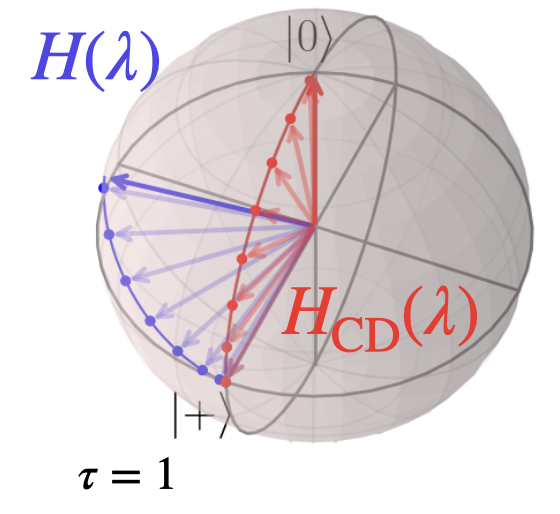
\includegraphics[width=0.9\linewidth]{images/rotating_spin_CD.png} \caption[Rotating spin Bloch sphere illustration with counterdiabatic driving]{State of the rotating spin starting in state $\ket{+}$ driven without \acrref{CD} as in the Hamiltonian of Eq.~\eqref{eq:rotating_spin_H_lambda} (blue) and with \acrref{CD} as given by Eq.~\eqref{eq:rotating_spin_HCD} (red) for total driving time $\tau = 1$.}\label{fig:rotating_CD}
    \end{wrapfigure}
    
    All that remains is to find $G_{\lambda}(\approxAGP)$ and to minimize the corresponding action $\mathcal{S}(\approxAGP)$ with respect to the driving coefficient $\alpha$. Once this process is complete (see App.~\ref{app:rotating_spin_hamiltonian} for details), we find that
    \begin{equation}\label{eq:rotating_spin_alpha}
        \alpha(\lambda) = -\frac{\sin^2(\lambda) + \cos^2(\lambda)}{2(\sin^2(\lambda) + \cos^2(\lambda))} = - \frac{1}{2},
    \end{equation}
    meaning that the counterdiabatic Hamiltonian can be written simply as:
    \begin{equation}\label{eq:rotating_spin_HCD}
        \begin{aligned}
            \HCD(\lambda) &= H(\lambda) + \dotlambda \alpha(\lambda) \sy \\
            &= -\cos(\lambda)\sx - \sin(\lambda)\sz - \frac{\pi}{4 \tau} \sy,
        \end{aligned}
    \end{equation}
    where we have used the fact that $\dotlambda = \pi/2\tau$. In Fig.~\ref{fig:rotating_CD}, we can see that even at very fast driving times, the rotating spin does not stray from the plane of rotation when the \acrref{CD} is applied. We can compare this to Fig.~\ref{fig:bloch_rotating_spin}, where similar dynamics without the application of a \acrref{CD} drive were only achieved at around $500$ times longer driving speeds.
    
    In this case, it turns out that the counterdiabatic term is constant as a result of the choice of basis and $H(\lambda)$. In general, however, this is not the case and the \acrref{CD} term depends on $\lambda$ through the coefficients of the lab frame Hamiltonian. Furthermore, while for this example only one operator was needed to describe the full \acrref{CD}, the number of such possible operators for a many-body system grows exponentially with system size, meaning that restricting to a highly-local and physically realisable basis is quite a sizeable reduction in the true number operators in the full \acrref{AGP}.
    
    \subsection{Nested commutator expansion}\label{sec:2.4.2_nested_commutators}

    The \acrref{LCD} approach is particularly useful in the case where one wants to implement a \acrref{CD} approximation constrained by some very limited, pre-determined set of operators, but it says absolutely nothing about what the operators should be when no constraints are imposed. A useful question to ask is whether or not there is any way to know what the operator basis of the approximate \acrref{CD} should be prior to performing the optimisation. This is useful not only in the case of determining the form of the \acrref{CD} in order to implement it, but also as a general tool in characterising non-adiabatic effects.

    In this section I will focus on an approach developed in \cite{claeys_floquet-engineering_2019}, where it was found that the \acrref{AGP} to some $\ell^{\rm th}$ order can be extracted from a series of nested commutators:
    \begin{equation}\label{eq:nested_commutator_AGP}
        \Bar{\AGP{\lambda}}^{(\ell)} = i\hbar \sum_{k=1}^\ell \alpha_k(\lambda) \underbrace{[H(\lambda),[H(\lambda),...[H(\lambda)}_{2k-1},\dlambda H(\lambda)]]],
    \end{equation}
    where the coefficients $\alpha_k(\lambda)$ are used in a similar manner as \acrref{LCD} and can be found for each set of operators at order $k$ using the minimisation procedure outlined in section \ref{sec:2.4.1_LCD}. In the limit of $\ell \rightarrow \infty$, the expression above should represent the exact \acrref{AGP}, although there is no guarantee of convergence prior to this point as during each iteration of the commutations, the set of operators that are obtained need not be orthogonal to the previous set. This means that even when the set of operators contains all the required degrees of freedom to describe the exact \acrref{AGP}, the minimisation procedure is hampered due to the lack of linearity that is readily available in the \acrref{LCD} approach.

    As noted in \cite{claeys_floquet-engineering_2019}, there are several ways to motivate this form of the \acrref{AGP}, \@e.g.~by noticing that such commutator terms appear in the Baker-Campbell-Hausdorff (BCH) expansion in the definition of a (properly regularized) \cite{jarzynski_geometric_1995} \acrref{AGP} for a fixed $\lambda$:
    \begin{equation}\label{eq:regularised_AGP}
        \AGP{\lambda} = \lim_{\epsilon \rightarrow 0^{+}} \int_0^{\infty} dt e^{-\epsilon t} \left( e^{-iH(\lambda) t}\dlambda H(\lambda)e^{iH(\lambda) t} + F_{\lambda} \right),
    \end{equation}
    where $F_{\lambda}$ is defined in Eq.~\eqref{eq:generalized_force_operator}. From the BCH expansion, we can find
    \begin{equation}
        e^{-iH t}\dlambda H e^{iH t} = \sum_{k = 0}^{\infty} \frac{(-it)^k}{k!} \underbrace{[H,[H,...[H}_{k},\dlambda H]]],
    \end{equation}
    where even-order commutators contribute to $F_{\lambda}$ and odd-order commutators to $\AGP{\lambda}$.
    
    To gain more intuition for Eq.~\eqref{eq:nested_commutator_AGP}, one can try to evaluate it in the instantaneous eigenbasis of $H(\lambda)$:
    \begin{equation}\label{eq:nested_commutator_matrix_elements}
        \begin{aligned}
            \mel*{m}{\Bar{\AGP{\lambda}}^{(\ell)}}{n} &= i\hbar \sum_{k=1}^\ell \alpha_k(\lambda) \mel*{m}{\underbrace{[H(\lambda),[H(\lambda),...[H(\lambda)}_{2k-1},\dlambda H(\lambda)]]]}{n} \\
            &= i\hbar \Bigg[ \sum_{k=1}^\ell \alpha_k(\lambda)(E_m - E_n)^{2k - 1} \Bigg] \mel{m}{\dlambda H}{n},
        \end{aligned}
    \end{equation}
    where we can see that the term we get out at the end looks very similar to the matrix elements we got in deriving the \acrref{AGP} in Eq.~\eqref{eq:differentiating_adiabatic_offdiagonals}. In the case of the nested commutator expansion then, the use of the variational \acrref{LCD} approach in determining the coefficients $\alpha_k$ is equivalent to trying to approximate the factor $(E_m - E_n)^{- 1}$ in the exact \acrref{AGP} via a power-series approximation:
    \begin{equation}
        \alpha_{\lambda}^{(\ell)}(\omega_{mn}) = \sum_{k=1}^\ell \alpha_k \omega_{mn}^{2k - 1},
    \end{equation}
    where $\omega_{mn} = (E_m - E_n)$. While this shows that the nested commutator approximation wouldn't work in regimes where the energy gap is exponentially small or exponentially big (\@i.e.~where $\omega_{mn} \rightarrow 0$ or $\omega_{mn} \rightarrow \infty$), this turns out to not be an issue in practice. In the limit of very large energy gaps, the term $\mel{m}{\dlambda H}{n}$ decays exponentially meaning that the contribution from these elements to the \acrref{AGP} is negligible anyway. As the energy gaps close, the \acrref{AGP} elements become undefined and generally in speeding up adiabatic processes, one only cares about suppressing transitions across some energy gap $\Delta$. In that case, as long as $\omega_{mn} \geq \Delta$, the approximation does its job in the \acrref{CD} protocol.

    In \cite{claeys_floquet-engineering_2019}, it was shown that the approximate \acrref{CD} Hamiltonians constructed using $\AGP{\lambda}^{(\ell)}$ can be implemented using Floquet Hamiltonians \cite{goldman_periodically_2014} by driving the $H$ and $\dlambda H$ terms at frequencies determined by the coefficients $\alpha_k$. However, for the purposes of this thesis, only the result presented in Eq.~\eqref{eq:nested_commutator_AGP} matters, as far as it allows one to identify operators in the \acrref{AGP} basis without requiring to make an ansatz with no further insight.